\documentclass[14pt]{extbook}
\usepackage{multicol, enumerate, enumitem, hyperref, color, soul, setspace, parskip, fancyhdr} %General Packages
\usepackage{amssymb, amsthm, amsmath, latexsym, units, mathtools} %Math Packages
\everymath{\displaystyle} %All math in Display Style
% Packages with additional options
\usepackage[headsep=0.5cm,headheight=12pt, left=1 in,right= 1 in,top= 1 in,bottom= 1 in]{geometry}
\usepackage[usenames,dvipsnames]{xcolor}
\usepackage{dashrule}  % Package to use the command below to create lines between items
\newcommand{\litem}[1]{\item#1\hspace*{-1cm}\rule{\textwidth}{0.4pt}}
\pagestyle{fancy}
\lhead{Module11M}
\chead{}
\rhead{Version B}
\lfoot{3819-8783}
\cfoot{}
\rfoot{test}
\begin{document}

\begin{enumerate}
\litem{
The temperature of an object, $T$, in a different surrounding temperature $T_s$ will behave according to the formula $T(t) = Ae^{kt} + T_s$, where $t$ is minutes, $A$ is a constant, and k is a constant. Use this formula and the situation below to construct a model that describes the uranium's temperature, $T$, based on the amount of time t (in minutes) that have passed. Choose the correct constant $k$ from the options below.
\begin{center}
    \textit{ Uranium is taken out of the reactor with a temperature of $130^{\circ}$ C and is placed into a $15^{\circ}$ C bath to cool. After 24 minutes, the uranium has cooled to $67^{\circ}$ C. }
\end{center}
\begin{enumerate}[label=\Alph*.]
\item \( k = -0.02806 \)
\item \( k = -0.04440 \)
\item \( k = -0.03818 \)
\item \( k = -0.02866 \)
\item \( \text{None of the above} \)

\end{enumerate} }
\litem{
A town has an initial population of 40000. The town's population for the next 10 years is provided below. Which type of function would be most appropriate to model the town's population?

\begin{tabular}{c|c|c|c|c|c|c|c|c|c}
\textbf{Year} &1 &2 &3 &4 &5 &6 &7 &8 &9\tabularnewline \hline
\textbf{Pop} &40024 &40058 &40092 &40126 &40144 &40178 &40212 &40246 &40264\end{tabular}\begin{enumerate}[label=\Alph*.]
\item \( \text{Linear} \)
\item \( \text{Exponential} \)
\item \( \text{Logarithmic} \)
\item \( \text{Non-Linear Power} \)
\item \( \text{None of the above} \)

\end{enumerate} }
\litem{
Determine the appropriate model for the graph of points below.
\begin{center}
    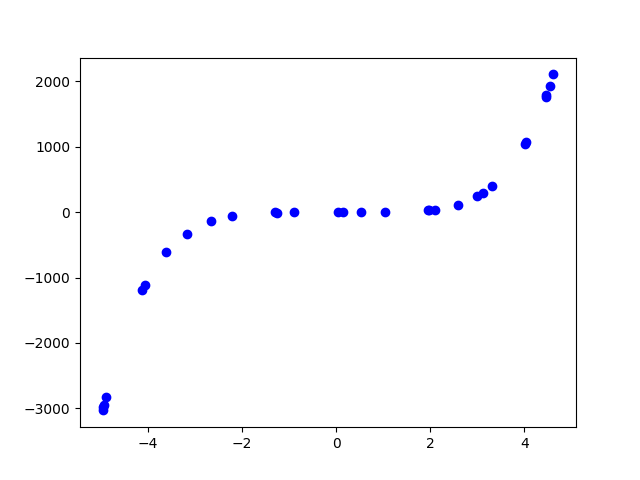
\includegraphics[width=0.5\textwidth]{../Figures/identifyModelGraph11B.png}
\end{center}
\begin{enumerate}[label=\Alph*.]
\item \( \text{Logarithmic model} \)
\item \( \text{Linear model} \)
\item \( \text{Non-linear Power model} \)
\item \( \text{Exponential model} \)
\item \( \text{None of the above} \)

\end{enumerate} }
\litem{
Determine the appropriate model for the graph of points below.
\begin{center}
    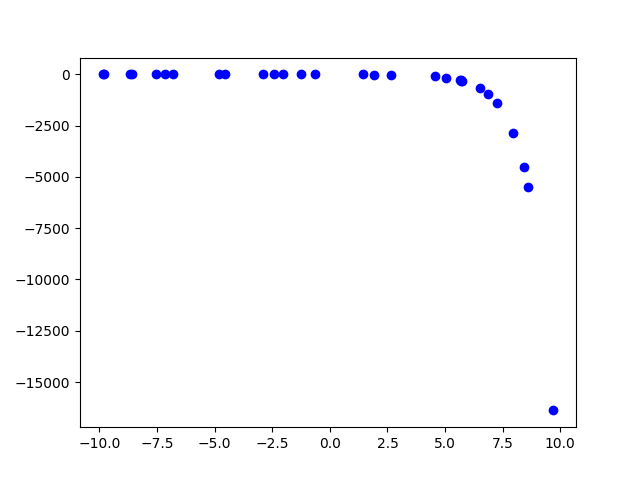
\includegraphics[width=0.5\textwidth]{../Figures/identifyModelGraph11CopyB.png}
\end{center}
\begin{enumerate}[label=\Alph*.]
\item \( \text{Exponential model} \)
\item \( \text{Non-linear Power model} \)
\item \( \text{Linear model} \)
\item \( \text{Logarithmic model} \)
\item \( \text{None of the above} \)

\end{enumerate} }
\litem{
Using the scenario below, model the situation using an exponential function and a base of $\frac{1}{2}$. Then, solve for the half-life of the element, rounding to the nearest day.
\begin{center}
    \textit{ The half-life of an element is the amount of time it takes for the element to decay to half of its initial starting amount. There is initially 607 grams of element $X$ and after 4 years there is 86 grams remaining. }
\end{center}
\begin{enumerate}[label=\Alph*.]
\item \( \text{About } 730 \text{ days} \)
\item \( \text{About } 0 \text{ days} \)
\item \( \text{About } 1825 \text{ days} \)
\item \( \text{About } 365 \text{ days} \)
\item \( \text{None of the above} \)

\end{enumerate} }
\litem{
The temperature of an object, $T$, in a different surrounding temperature $T_s$ will behave according to the formula $T(t) = Ae^{kt} + T_s$, where $t$ is minutes, $A$ is a constant, and k is a constant. Use this formula and the situation below to construct a model that describes the uranium's temperature, $T$, based on the amount of time t (in minutes) that have passed. Choose the correct constant $k$ from the options below.
\begin{center}
    \textit{ Uranium is taken out of the reactor with a temperature of $180^{\circ}$ C and is placed into a $14^{\circ}$ C bath to cool. After 31 minutes, the uranium has cooled to $140^{\circ}$ C. }
\end{center}
\begin{enumerate}[label=\Alph*.]
\item \( k = -0.01151 \)
\item \( k = -0.00889 \)
\item \( k = -0.02553 \)
\item \( k = -0.02519 \)
\item \( \text{None of the above} \)

\end{enumerate} }
\litem{
Using the scenario below, model the situation using an exponential function and a base of $\frac{1}{2}$. Then, solve for the half-life of the element, rounding to the nearest day.
\begin{center}
    \textit{ The half-life of an element is the amount of time it takes for the element to decay to half of its initial starting amount. There is initially 932 grams of element $X$ and after 3 years there is 93 grams remaining. }
\end{center}
\begin{enumerate}[label=\Alph*.]
\item \( \text{About } 0 \text{ days} \)
\item \( \text{About } 365 \text{ days} \)
\item \( \text{About } 1460 \text{ days} \)
\item \( \text{About } 0 \text{ days} \)
\item \( \text{None of the above} \)

\end{enumerate} }
\litem{
A town has an initial population of 60000. The town's population for the next 10 years is provided below. Which type of function would be most appropriate to model the town's population?

\begin{tabular}{c|c|c|c|c|c|c|c|c|c}
\textbf{Year} &1 &2 &3 &4 &5 &6 &7 &8 &9\tabularnewline \hline
\textbf{Pop} &60000 &59965 &59945 &59930 &59919 &59910 &59902 &59896 &59890\end{tabular}\begin{enumerate}[label=\Alph*.]
\item \( \text{Exponential} \)
\item \( \text{Non-Linear Power} \)
\item \( \text{Logarithmic} \)
\item \( \text{Linear} \)
\item \( \text{None of the above} \)

\end{enumerate} }
\litem{
Using the scenario below, model the population of bacteria $\alpha$ in terms of the number of minutes, $t$ that pass. Then, choose the correct approximate \textit{(rounded to the nearest minute)} replication rate of bacteria-$\alpha$.
\begin{center}
    \textit{ A newly discovered bacteria, $\alpha$, is being examined in a lab. The lab started with a petri dish of 2 bacteria-$\alpha$. After 1 hours, the petri dish has 7 bacteria-$\alpha$. Based on similar bacteria, the lab believes bacteria-$\alpha$ doubles after some undetermined number of minutes. }
\end{center}
\begin{enumerate}[label=\Alph*.]
\item \( \text{About } 53 \text{ minutes} \)
\item \( \text{About } 319 \text{ minutes} \)
\item \( \text{About } 49 \text{ minutes} \)
\item \( \text{About } 298 \text{ minutes} \)
\item \( \text{None of the above} \)

\end{enumerate} }
\litem{
Using the scenario below, model the population of bacteria $\alpha$ in terms of the number of minutes, $t$ that pass. Then, choose the correct approximate \textit{(rounded to the nearest minute)} replication rate of bacteria-$\alpha$.
\begin{center}
    \textit{ A newly discovered bacteria, $\alpha$, is being examined in a lab. The lab started with a petri dish of 2 bacteria-$\alpha$. After 2 hours, the petri dish has 5176 bacteria-$\alpha$. Based on similar bacteria, the lab believes bacteria-$\alpha$ quadruples after some undetermined number of minutes. }
\end{center}
\begin{enumerate}[label=\Alph*.]
\item \( \text{About } 116 \text{ minutes} \)
\item \( \text{About } 63 \text{ minutes} \)
\item \( \text{About } 10 \text{ minutes} \)
\item \( \text{About } 19 \text{ minutes} \)
\item \( \text{None of the above} \)

\end{enumerate} }
\end{enumerate}

\end{document}